\documentclass[a4paper,10pt]{ltjsarticle}

% 各種字体
% cf. http://www.yamamo10.jp/yamamoto/comp/latex/make_doc/formula/amsmath_symbol/index.php
\usepackage{amsmath,amssymb,amsfonts}

% 画像挿入
\usepackage{graphicx}
% 表のボーダー
\usepackage{booktabs}
% ハイパーリンク, URL 挿入
\usepackage{hyperref,url}
% 色付き文字
\usepackage{xcolor}

% 改ページできるフレーム
\usepackage{framed}

% 単位
% cf. http://www.yamamo10.jp/yamamoto/comp/latex/make_doc/unit/index.php
\usepackage{siunitx}

\usepackage{tikz}
\usetikzlibrary{
  shapes.misc,
  arrows.meta,
  decorations,
  decorations.markings
}

%-----------%
% スニペット %
%-----------%

% cf. https://mirrors.ctan.org/macros/latex/contrib/physics2/physics2.pdf
% cf. https://ctan.uib.no/macros/latex/contrib/physics2/physics2-legacy.pdf

\usepackage{physics2}
% 自動調整の括弧:\ab() など
\usephysicsmodule{ab}

% 微小量記号:\d など
\usepackage{fixdif}
% 微分記号:\pdv など
\usepackage{derivative}

\usepackage{braket}

\makeatletter
\newcommand\vb{\@ifstar\boldsymbol\mathbf}
\newcommand\va[1]{\@ifstar{\vec{#1}}{\vec{\mathrm{#1}}}}
\newcommand\vu[1]{% 
  \@ifstar{\hat{\boldsymbol{#1}}}{\hat{\mathbf{#1}}}}
\makeatother

%-----------%
% コード関連 %
%-----------%

% 疑似コード
% cf. https://tug.ctan.org/macros/latex/contrib/algorithmicx/algorithmicx.pdf
% cf. https://qiita.com/tomoyk/items/6016123b5c9034bb0087
\usepackage{algorithm}
\usepackage{algpseudocode}

% コードブロック
% cf. https://cloudlatex.io/latex-notation#%E3%82%BD%E3%83%BC%E3%82%B9%E3%82%B3%E3%83%BC%E3%83%89
\usepackage{listings}
% \usepackage{jvlisting}

% Global style setting
% cf. https://nasa.github.io/nasa-latex-docs/html/examples/listing.html
\lstset{
  language={C}, % 載せるソースコードの言語を指定する
  basicstyle={\small}, % 通常のソースのフォントを設定
  identifierstyle={\small},% 変数名などのフォントを設定
  commentstyle={\small\itshape\color[rgb]{0,0.5,0}}, % コメントのフォントを設定
  keywordstyle={\small\bfseries\color[rgb]{0,0,1}}, % 予約語のフォントを設定
  ndkeywordstyle={\small}, % keywordstyle以外に定義されている予約語のフォントを設定
  stringstyle={\small\ttfamily\color[rgb]{1,0,1}}, % 文字列のフォントを設定
  frame={tb}, % 実線で描く枠の位置指定
  breaklines=true, % 自動改行の有無
  columns=[l]{fullflexible},% 文字間の余白
  numbers=left, % 行番号の位置
  numberstyle={\scriptsize}, % 行番号のフォント
  stepnumber=1, % 行番号の刻み幅
  lineskip=-0.5ex, % 行間
}

% インラインコードブロック (\lstinline)
% cf. https://tex.stackexchange.com/questions/357227/adding-background-color-to-verb-or-lstinline-command-without-colorbox
\usepackage{xpatch}
\usepackage{realboxes}
\definecolor{mygray}{rgb}{0.95,0.95,0.95}
\makeatletter
\xpretocmd\lstinline{\Colorbox{mygray}\bgroup\appto\lst@DeInit{\egroup}}{}{}
\makeatother

%---------%
% 参考文献 %
%---------%

% cf. https://tex.stackexchange.com/questions/655812/how-to-include-a-url-in-a-customized-way-with-unsrt
\usepackage[numbers, sort]{natbib}
\bibliographystyle{unsrtnat}

%---------------%
% 適宜切り替える %
%---------------%

% 、。と ,. の切り替え (LuaLaTeX 専用)
\usepackage{newunicodechar}
\newunicodechar{、}{,}
\newunicodechar{。}{.}

% ページ数を消す
% \pagestyle{empty}

%---------%
% 文章情報 %
%---------%

\title{堀田量子第9章ノート}
\author{山崎 雅史}

\begin{document}

\maketitle
\begin{abstract}
  堀田量子~\cite{hotta2021qm}の第9章に基づいて
  量子化された調和振動子のハミルトニアンの構成と
  シュレディンガー方程式の立式を行う。
  また量子調和振動子の伝搬関数に対する天下りの公式による確認と、
  経路積分を用いた導出~\cite{osborn2014aqft}もする。
\end{abstract}
\tableofcontents

\setcounter{section}{8}

\section{量子調和振動子}

\setcounter{subsection}{-1}


\subsection{使用する公式の復習}

昇降演算子 (ladder operator) $\hat{a},\hat{a}^\dagger$のリー代数は次の式。
\begin{equation}
  \label{eq:a_algebra}
  [\hat{a},\hat{a}^\dagger] = 1
  \tag{8.15}
\end{equation}
% textlint-disable
エルミート演算子
\begin{equation}
  \hat{N}\equiv\hat{a}^\dagger\hat{a} \tag{8.7}
\end{equation}
と昇降演算子$\hat{a},\hat{a}^\dagger$のリー代数は次の式。
% textlint-enable
\begin{equation}
  \begin{split}
    &[\hat{N},\hat{a}^\dagger]
    =\hat{a}^\dagger[\hat{a},\hat{a}^\dagger]
    =\hat{a}^\dagger, \\
    &[\hat{N},\hat{a}]
    =[\hat{a}^\dagger\hat{a},\hat{a}]
    =[\hat{a}^\dagger,\hat{a}]\hat{a}
    =-\hat{a}
  \end{split}
\end{equation}
このリー代数に対する$N-1$を最高ウェイトとする既約表現をもつ。
これを最高ウェイト表現と呼ぶ。
線形空間$\ab\{\sum_{i=0}^{N-1}k_i\ket{i}|k_i\in\mathbb{C}\}$に対する表現は次の式。
\begin{align}
   & \hat{a}\ket{N-1} = 0                       \\
   & \hat{a}^\dagger\ket{n}=\sqrt{n+1}\ket{n+1}
  \quad(n=0,1,\ldots,N-2)
  \tag{8.2}                                     \\
   & \hat{a}\ket{n}=\sqrt{n}\ket{n-1}
  \quad(n=1,\ldots,N-1)
  \tag{8.5}                                     \\
   & \hat{N}\ket{n}=n\ket{n}
  \tag{8.8}
  \label{eq:number_op_repr}
\end{align}
この表現から線形空間の基底が次の式で書ける。
\begin{equation}
  \label{eq:num_eigenvec}
  \ket{n}
  =\frac{1}{\sqrt{n!}}(\hat{a}^\dagger)^n\ket{0}
  \tag{8.4}
\end{equation}

位置演算子$\hat{x}$、運動量演算子$\hat{p}$の交換関係は以下。
\begin{equation}
  \label{eq:xp_alg}
  [\hat{x},\hat{p}]=i\hbar
  \tag{8.18}
\end{equation}
系を特徴づける長さ$L$を用いると
位置演算子$\hat{x}$、運動量演算子$\hat{p}$から
昇降演算子$\hat{a},\hat{a}$のリー代数をもつ演算子が作れる。
\begin{equation}
  \label{eq:xp2a}
  \hat{a}=\frac{1}{\sqrt{2}}
  \ab(\frac{\hat{x}}{L}+i\frac{L\hat{p}}{\hbar}),\quad
  \hat{a}^\dagger=\frac{1}{\sqrt{2}}
  \ab(\frac{\hat{x}}{L}-i\frac{L\hat{p}}{\hbar})
  \tag{8.17}
\end{equation}
ただし昇降演算子$\hat{a},\hat{a}^\dagger$は無次元量。
% textlint-disable
これは換算プランク定数あるいは Dirac 定数が
\begin{equation}
  \begin{split}
    \hbar\equiv\frac{h}{2\pi}
    &= 1.054571817\ldots\times10^{-34}\si{J.s} \\
    &= 6.582119569\ldots\times10^{-16}\si{eV.s}
  \end{split}
\end{equation}
と定義され、運動エネルギー$K$の公式に対する次元解析が
\begin{equation}
  K=\frac{1}{2}mv^2
  \Rightarrow[K]=ML^2T^{-2}
\end{equation}
となることから
\begin{equation}
  \ab[\frac{Lp}{\hbar}]
  =\frac{[L][p]}{[\hbar]}
  =\frac{L\cdot MLT^{-1}}{ML^2T^{-2}\cdot T}
  = 1
\end{equation}
となって無次元になることが確かめられる。
% textlint-enable
逆に昇降演算子$\hat{a},\hat{a}^\dagger$から
位置・運動量の単位をもつ次の演算子が定義できる。
\begin{equation}
  \label{eq:a2xp}
  \hat{x}=\frac{L}{\sqrt{2}}(\hat{a}+\hat{a}^\dagger),\quad
  \hat{p}=\frac{\hbar}{\sqrt{2}iL}(\hat{a}-\hat{a}^\dagger)
  \tag{8.16}
\end{equation}

孤立系$S$のハミルトニアン$\hat{H}_S$から定まる
状態$\ket{\psi(t)}_S$の時間発展は
次のシュレディンガー方程式で記述される。
\begin{equation}
  \label{eq:schrodinger_eq}
  i\hbar\odv{}{t}\ket{\psi(t)}_S
  =\hat{H}_S(t)\ket{\psi(t)}_S
  \tag{6.18}
\end{equation}
このように状態を時間依存させる記法を
シュレディンガー描像と呼ぶ。

孤立系$S$のハミルトニアン$\hat{H}_S$から定まる
ハイゼンベルグ演算子$\hat{O}_H(t)$の時間発展は
次のハイゼンベルグ方程式で記述される。
\begin{equation}
  \label{eq:heisenberg_eq}
  \odv{}{t}\hat{O}_H(t)
  =\frac{1}{i\hbar}\ab[\hat{O}_H(t),\hat{H}_H(t)]
  \tag{6.36}
\end{equation}
このように演算子を時間依存させる記法を
ハイゼンベルク描像と呼ぶ。

運動量演算子の位置表示はデルタ関数の微分。
\begin{equation}
  \label{eq:p_in_x}
  \braket{x|\hat{p}|x'}
  =-i\hbar\pdv{}{x}\delta(x-x')
  \tag{8.41}
\end{equation}
波動関数$\psi(x)=\braket{x|\psi}$に作用する位置表示の
運動量演算子と位置演算子は次で定義。
\begin{equation}
  \vb{p}=-i\hbar\pdv{}{x},\quad
  \vb{x}=x
  \tag{8.43}
\end{equation}
これは次の意味。
\begin{equation}
  \begin{split}
    &\hat{p}\ket{p}=p\ket{p}
    \Rightarrow
    \braket{x|\hat{p}|p}
    =p\braket{x|p} \\
    &\Leftrightarrow
    p\braket{x|p}
    =\braket{x|\hat{p}|p}
    =\int_{-\infty}^\infty\d x'
    \braket{x|\hat{p}|x'}\braket{x'|p}
    =\int_{-\infty}^\infty\d x'
    \ab(-i\hbar\pdv{}{x}\delta(x-x'))\braket{x'|p} \\
    &\quad\,=
    -i\hbar\pdv{}{x}
    \int_{-\infty}^\infty\d x'
    \delta(x-x')\braket{x'|p}
    =-i\hbar\pdv{}{x}\braket{x|p}
    =\vb{p}\braket{x|p}
  \end{split}
\end{equation}

\subsection{ハミルトニアン}

昇降演算子$\hat{a},\hat{a}^\dagger$からハミルトニアン$H$を構築する。
ハミルトニアン$H$はエネルギーの次元をもつエルミート演算子である。
昇降演算子$\hat{a},\hat{a}^\dagger$は無次元であったから、
ハミルトニアンの構築にはエネルギーの次元をもつ定数を導入する必要がある。
量子効果を表すために換算プランク定数$\hbar$を含む必要があるので、
これと組み合わせてエネルギーの次元をもつ定数を構成できるよう
時間の逆数の次元をもつ角振動数$\omega$を導入する。
つまりエネルギーの次元をもつ定数$\hbar\omega$をハミルトニアン$H$の構築に使う。

昇降演算子$\hat{a},\hat{a}^\dagger$で構成される
もっとも一般的な演算子$A$は次の式で書かれる (ansatz)。
\begin{equation}
  \label{eq:A_ansatz}
  A=\sum_{m=0}^\infty\sum_{n=0}^\infty c_{mn}(\hat{a}^\dagger)^m\hat{a}^n
\end{equation}
% textlint-disable
$\hat{a}\hat{a}^\dagger\hat{a}$など他の順序の積をもつ項についても、
交換関係 (\ref{eq:a_algebra}) 式を用いて$\hat{a}^\dagger$を
左に移動させれば (\ref{eq:A_ansatz}) 式と同じ形に帰着させることができる。
% textlint-enable
このうちエルミートとなるものは次の条件を満たす場合。
\begin{equation}
  \label{eq:hermitian_constraint}
  A=A^\dagger
  \Leftrightarrow
  c_{mn} = c^\ast_{nm}
\end{equation}
よって昇降演算子$\hat{a},\hat{a}^\dagger$を用いる
ハミルトニアン$H$の一般形は次の式になる。
\begin{equation}
  \label{eq:H_ansatz}
  H=
  \sum_{m=0}^\infty c_{mm}\hat{N}^m
  +\sum_{m>n\geq0} c_{mn}(\hat{a}^\dagger)^m\hat{a}^n
  +\sum_{n>m\geq0} c^\ast_{nm}(\hat{a}^\dagger)^m\hat{a}^n,\quad
  c_{mm}\in\mathbb{R}
\end{equation}
ただし交換関係 (\ref{eq:a_algebra}) 式を用いたあとに$c_{00}$を再定義した。
系の安定性を考えて固有値に下限をもつハミルトニアンに限ると
一般形はさらに絞り込むことができる。
(\ref{eq:hermitian_constraint})式を用いると$m>n$の場合で次が分かる。
\begin{equation}
  \label{eq:hermitian_decomposite}
  \begin{split}
    &c_{mn}(\hat{a}^\dagger)^m\hat{a}^n
    + c_{nm}(\hat{a}^\dagger)^n\hat{a}^m
    =c_{mn}(\hat{a}^\dagger)^m\hat{a}^n
    + c^\ast_{mn}(\hat{a}^\dagger)^n\hat{a}^m \\
    &=\hat{N}^n
    (c_{mn}(\hat{a}^\dagger)^{m-n}+c^\ast_{mn}\hat{a}^{m-n})
    +\text{const.} \\
    &=\hat{N}^n
    \ab[
      \Re(c_{mn})\ab((\hat{a}^\dagger)^{m-n}+\hat{a}^{m-n})
      +i\Im(c_{mn})\ab((\hat{a}^\dagger)^{m-n}-\hat{a}^{m-n})
    ]+\text{const.}
  \end{split}
\end{equation}
(\ref{eq:H_ansatz})(\ref{eq:hermitian_decomposite})(\ref{eq:xp2a})
式を合わせることで
次を得る。
\begin{equation}
  \begin{split}
    H &= c'_{00} +
    \Re(c_{10})\ab(\hat{a}^\dagger+\hat{a})
    +i\Im(c_{10})\ab(\hat{a}^\dagger-\hat{a})
    +c_{11}\hat{N} \\
    &\quad+\hat{N}
    \ab[
      \Re(c_{20})\ab((\hat{a}^\dagger)^2+\hat{a}^2)
      +i\Im(c_{20})\ab((\hat{a}^\dagger)^2-\hat{a}^2)
    ]
    +\ldots \\
    &= c'_{00} +
    \Re(c_{10})\frac{\sqrt{2}\hat{x}}{L}
    -\Im(c_{10})\frac{\sqrt{2}L\hat{p}}{\hbar}
    +c_{11}\hat{N} \\
    &\quad+\hat{N}
    \ab[\Re(c_{20})
      \ab(
      \frac{\hat{x}^2}{L^2}-\frac{L^2\hat{p}^2}{\hbar^2}
      )
      +\Im(c_{20})
      \frac{1}{\hbar}(\hat{x}\hat{p}+\hat{p}\hat{x})
    ]
    +\ldots
  \end{split}
\end{equation}
ただし定数項を$c_{00}'$に吸収させた。
ここで$\hat{x},\hat{p}$の固有値の値域は
$[-\infty,\infty]$であるから、
$H$からこれらの$-\infty$の固有値を取りうる項を除外するために
次の条件が必要になる。
\begin{equation}
  c_{10}=c_{20}=\ldots=0
\end{equation}
よってハミルトニアン$H$がエルミートで固有値に下限をもつことから
次の一般形を得る。
\begin{equation}
  \hat{H}
  =c'_{00}+c_{11}\hat{N}+\ldots,\quad
  c_{mm}\in\mathbb{R}
\end{equation}
このうち非自明でもっとも簡単なケースは次のケースである。
\begin{equation}
  c'_{11}\neq0,\quad
  c_{mn} = 0\quad(m\geq2\quad\text{or}\quad n\geq2)
\end{equation}
ここで係数$c'_{00},c_{11}$は前述のようにエネルギーの次元をもつように
$\hbar\omega$に比例させるように定義する。
慣例にもとづき比例係数については次のように選ぶ。
\begin{equation}
  \label{eq:ladder_H}
  \hat{H}
  =\frac{\hbar\omega}{2}\ab(\hat{a}^\dagger\hat{a}+\hat{a}\hat{a}^\dagger)
  =\hbar\omega\ab(\hat{a}^\dagger\hat{a}+\frac{1}{2})
  \tag{9.1}
\end{equation}
(\ref{eq:number_op_repr}) 式を用いれば
このハミルトニアン$H$が次の固有値をもつことが分かる。
\begin{equation}
  E_n=\hbar\omega\ab(\omega+\frac{1}{2}),\quad
  n=0,1,2,\ldots
\end{equation}

エネルギースペクトラムの離散性は古典領域$n\gg1$で無視できる。
これはエネルギー準位の相対的な増分が次の式であることから分かる。
\begin{equation}
  \frac{\Delta E}{E} = \frac{1}{n+\frac{1}{2}}
  \overset{n\rightarrow\infty}{\longrightarrow}0
\end{equation}

$\omega$ は現象に応じてさまざまな値をとる。
たとえば共振器オプトメカニクス (Cavity optomechanics) では
レーザ(フォトン)と機械振動(フォノン)の相互作用で量子的な調和振動子を再現する。
観測できる物理量はフォノン側である。
図~\ref{fig:FigureOptomechanicalSystem}に共振オプトメカニクスの概要を示す。
\begin{figure}[tbp]
  \begin{center}
    \includegraphics[width=8cm]{img/FigureOptomechanicalSystem.pdf}
    \caption{共振器オプトメカニクスの概要~\cite{aspelmeyer2014cavity}}\label{fig:FigureOptomechanicalSystem}
  \end{center}
\end{figure}
量子的な光共振器 (optical cavity) の物理量を力学現象のモード (mechanical mode) を通じて観測する。
共振器オプトメカニクスの構造をもつ現象は複数知られており、
これまでに実施された実験を図~\ref{fig:Figure_Overview_OptomechanicsFinal}に示す。
\begin{figure}[tbp]
  \begin{center}
    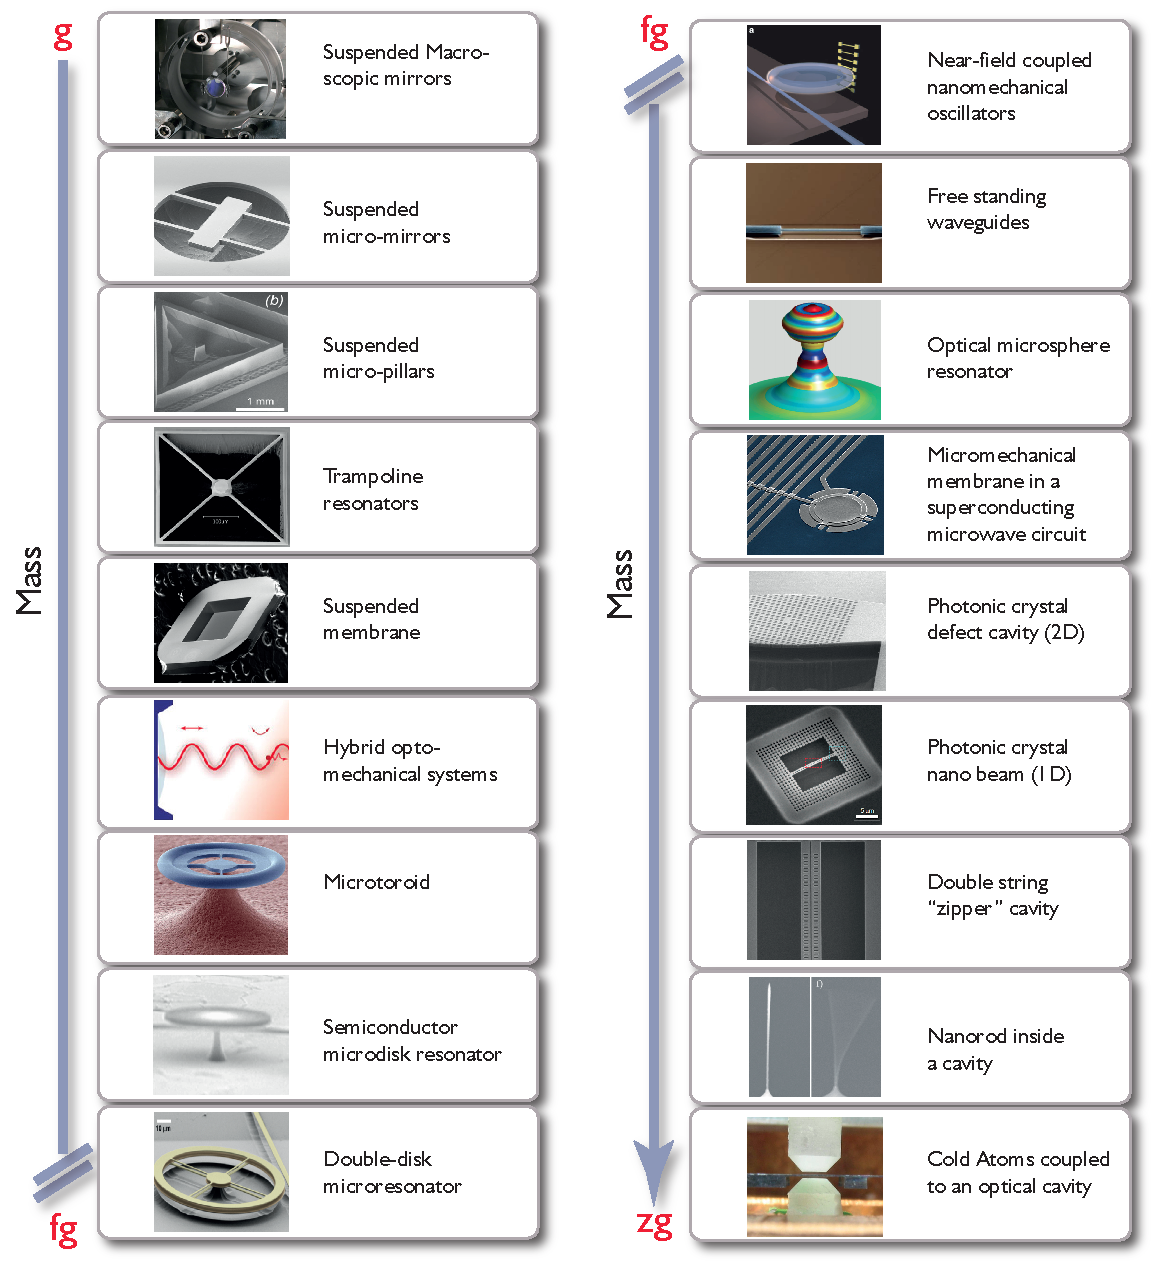
\includegraphics[width=11cm]{img/Figure_Overview_OptomechanicsFinal.png}
    \caption{共振器オプトメカニクスの実験例}\label{fig:Figure_Overview_OptomechanicsFinal}
  \end{center}
\end{figure}
この図では実験に使用されている調和振動子の質量の大きさ$m$でソートされている。
質量単位はフェムトグラム$\si{fg}=10^{-15}\si{g}$がゼプトグラム$\si{zg}=10^{-21}\si{g}$使われている。
共振器オプトメカニクスの実験で観測されている
フォノンの角振動数$\omega$あるいは$\Omega_m$は
図~\ref{fig:cavity_optomechanics_example_table}のとおりである。
\begin{figure}[tbp]
  \begin{center}
    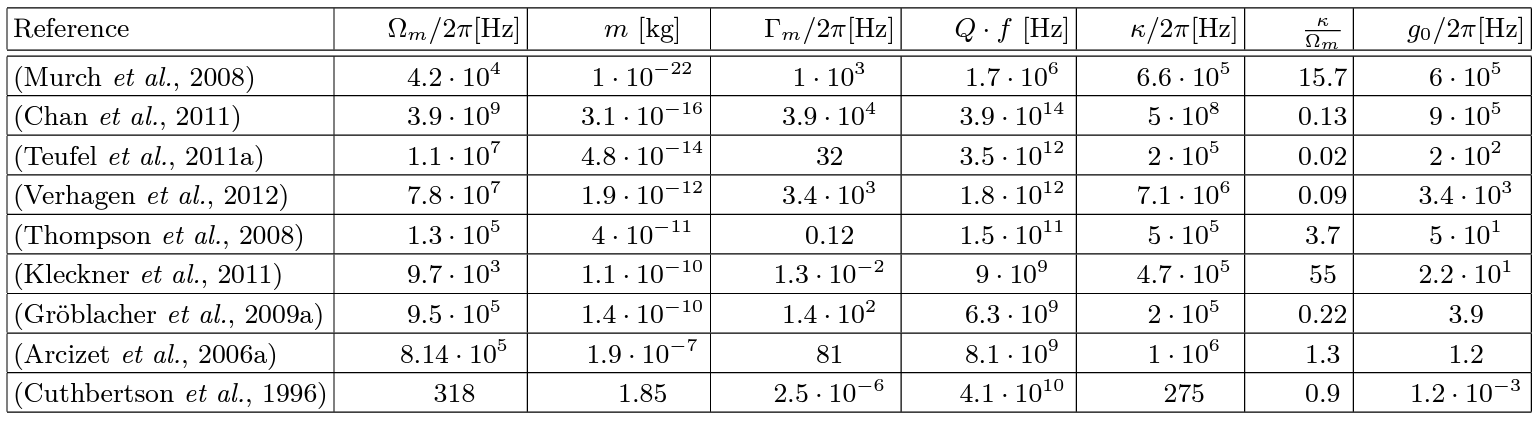
\includegraphics[width=15cm]{img/cavity_optomechanics_example_table.png}
    \caption{共振器オプトメカニクスの実験におけるパラメータ一覧~\cite{aspelmeyer2014cavity}}\label{fig:cavity_optomechanics_example_table}
  \end{center}
\end{figure}
角振動数$\omega$の取りうる単位はおおむね$10^2\sim10^9\si{Hz}$のオーダーである。
この場合$\hbar\omega$の値は$10^{-14}\sim10^{-7}\si{eV}$ほどになる。
$1\si{eV}$は電子1個が$1\si{V}$の電位差から得る位置エネルギーを指す。
また図~\ref{fig:cavity_optomechanics_example_table}から系の特徴的な長さ$L$が次の式で計算可能である。
\begin{equation}
  \label{eq:L_estimate}
  L=\sqrt{\frac{\hbar}{m\omega}}
  \tag{9.3}
\end{equation}
この式で特徴的長さ$L$が見積もれることは次の次元解析から分かる。
\begin{equation}
  [\hbar\omega]=[E]=[mc^2]=ML^2T^{-2}
  \Rightarrow
  \ab[\frac{\hbar}{m\omega}]
  =\ab[\frac{\hbar\omega}{m\omega^2}]
  = ML^2T^{-2}(MT^{-2})^{-1}=L^2
\end{equation}
図~\ref{fig:cavity_optomechanics_example_table}のケースでは
特徴的長さ$L$は$1\si{am}\sim1\si{nm}$程である。

昇降演算子によるハミルトニアン (\ref{eq:ladder_H}) 式の
位置・運動量演算子$\hat{x},\hat{p}$による表示を得るには
(\ref{eq:a2xp})式を用いて次のように変形すればよい。
\begin{equation}
  \begin{split}
    \hat{H}
    &=\hbar\omega\ab(\hat{a}^\dagger\hat{a}+\frac{1}{2})
    =\hbar\omega\ab[
      \frac{1}{\sqrt{2}}
      \ab(\frac{\hat{x}}{L}-i\frac{L\hat{p}}{\hbar})
      \cdot
      \frac{1}{\sqrt{2}}
      \ab(\frac{\hat{x}}{L}+i\frac{L\hat{p}}{\hbar})
      +\frac{1}{2}
    ] \\
    &=\frac{\hbar\omega}{2}\ab[
      \frac{\hat{x}^2}{L^2}
      -\frac{1}{i\hbar}(\hat{x}\hat{p}-\hat{p}\hat{x})
      +\frac{L^2\hat{p}^2}{\hbar^2}
      +1
    ] \\
    &=\frac{\hbar\omega}{2}\ab[
      \frac{\hat{x}^2}{L^2}
      +\frac{L^2\hat{p}^2}{\hbar^2}
    ]
  \end{split}
\end{equation}
ただし位置・運動量演算子$\hat{x},\hat{p}$の交換関係 (\ref{eq:xp_alg}) 式を用いた。
特徴的長さ$L$の推定 (\ref{eq:L_estimate}) 式を代入すると次の結果を得る。
\begin{equation}
  \label{eq:H_xp}
  \hat{H}=\frac{1}{2m}\hat{p}^2+\frac{m\omega^2}{2}\hat{x}^2
  \tag{9.4}
\end{equation}
実際には$L$の式は推定に過ぎないので$\mathcal{O}(1)$の不定性があるが、
$m,\omega$の再定義や単位系の取り直しで吸収したこととする。

位置・運動量に関するハイゼンベルグ演算子は次の式で定義される。
\begin{equation}
  \begin{split}
    \hat{x}_H
    &=\exp\ab(\frac{it}{\hbar}\hat{H})\hat{x}\exp\ab(-\frac{it}{\hbar}\hat{H}), \\
    \hat{p}_H
    &=\exp\ab(\frac{it}{\hbar}\hat{H})\hat{p}\exp\ab(-\frac{it}{\hbar}\hat{H})
  \end{split}
  \tag{9.5}
\end{equation}
これらの時間発展はハミルトニアン$\hat{H}$による
ハイゼンベルグ方程式 (\ref{eq:heisenberg_eq}) 式から求まる。
位置演算子$\hat{x}_H(t)$の時間発展は次のとおりである。
\begin{equation}
  \begin{split}
    &\odv{}{t}\hat{x}_H(t)
    =\frac{1}{i\hbar}\ab[\hat{x}_H(t),\hat{H}]
    =\frac{1}{i\hbar}
    \ab[
      \exp\ab(\frac{it}{\hbar}\hat{H})
      \hat{x}
      \exp\ab(-\frac{it}{\hbar}\hat{H}),
      \hat{H}
    ] \\
    &=\frac{1}{i\hbar}
    \exp\ab(\frac{it}{\hbar}\hat{H})
    \ab[\hat{x},\hat{H}]
    \exp\ab(-\frac{it}{\hbar}\hat{H})
    \\
    &=\frac{1}{i\hbar}
    \exp\ab(\frac{it}{\hbar}\hat{H})
    \ab[
      \hat{x},\frac{1}{2m}\hat{p}^2+\frac{m\omega^2}{2}\hat{x}^2
    ]
    \exp\ab(-\frac{it}{\hbar}\hat{H})
    \\
    &=\frac{1}{i\hbar}
    \exp\ab(\frac{it}{\hbar}\hat{H})
    \frac{1}{2m}
    \ab(\ab[\hat{x},\hat{p}]\hat{p}+\hat{p}\ab[\hat{x},\hat{p}])
    \exp\ab(-\frac{it}{\hbar}\hat{H})\\
    &=\frac{1}{m}\hat{p}_H(t)
  \end{split}
\end{equation}
運動量演算子$\hat{p}_H(t)$の時間発展は次のとおりである。
\begin{equation}
  \begin{split}
    &\odv{}{t}\hat{p}_H(t)
    =\frac{1}{i\hbar}\ab[\hat{p}_H(t),\hat{H}]
    =\frac{1}{i\hbar}
    \ab[
      \exp\ab(\frac{it}{\hbar}\hat{H})
      \hat{p}
      \exp\ab(-\frac{it}{\hbar}\hat{H}),
      \hat{H}
    ] \\
    &=\frac{1}{i\hbar}
    \exp\ab(\frac{it}{\hbar}\hat{H})
    \ab[\hat{p},\hat{H}]
    \exp\ab(-\frac{it}{\hbar}\hat{H})
    \\
    &=\frac{1}{i\hbar}
    \exp\ab(\frac{it}{\hbar}\hat{H})
    \ab[
      \hat{p},\frac{1}{2m}\hat{p}^2+\frac{m\omega^2}{2}\hat{x}^2
    ]
    \exp\ab(-\frac{it}{\hbar}\hat{H})
    \\
    &=\frac{1}{i\hbar}
    \exp\ab(\frac{it}{\hbar}\hat{H})
    \frac{m\omega^2}{2}
    \ab(\ab[\hat{p},\hat{x}]\hat{p}+\hat{p}\ab[\hat{p},\hat{x}])
    \exp\ab(-\frac{it}{\hbar}\hat{H})\\
    &=-m\omega^2\hat{x}_H(t)
  \end{split}
\end{equation}
結果をまとめると次のとおりである。
\begin{equation}
  \begin{split}
    &\odv{}{t}\hat{x}_H(t)=\frac{1}{m}\hat{p}_H(t), \\
    &\odv{}{t}\hat{p}_H(t)=-m\omega^2\hat{x}_H(t)
  \end{split}
  \tag{9.6}
\end{equation}
この式は古典論の調和振動子の正準方程式と対応している。
これは古典論ではハミルトニアンがポアソン括弧における時間発展の生成子になっていることと、
ハイゼンベルク方程式に対応があることからも分かる。
よって (\ref{eq:H_xp}) 式は量子的な調和振動子のハミルトニアンであることが直感的に分かる。

(\ref{eq:H_xp}) 式のハミルトニアンを構成する際に、
昇降演算子$\hat{a}^\dagger,\hat{a}$の高次項を0とした。
(\ref{eq:a2xp}) 式を用いると$\hat{x},\hat{p}$の高次項を0としたことが分かる。
これは非線形相互作用を線形化あるいは無視した状況に対応する。
このようなハミルトニアン$\hat{H}$は線形応答を解析する際に現れる。

基底状態はエネルギー0ではなく次の零点エネルギー (zero-point energy) をもつ。
\begin{equation}
  \hat{H}\ket{0} = \frac{1}{2}\hbar\omega\ket{0}
\end{equation}
零点エネルギーが生じる理由は$\Delta x,\Delta p$ に関する次のケナード不等式によるものである。
\begin{equation}
  \Delta x \Delta p\geq\frac{\hbar}{2}
\end{equation}
ハミルトニアン$H$に対する固有値であるエネルギー準位の下限は
ケナード不等式の下限$\Delta x\Delta p=\dfrac{\hbar}{2}$で評価できる。
(\ref{eq:H_xp}) 式の各項の不確定性を考えることで次のように評価できる。
\begin{equation}
  E(\Delta x)
  =\frac{1}{2m}\Delta p^2+\frac{m\omega^2}{2}\Delta x^2
  \geq2\sqrt{\frac{1}{2m}\Delta p^2\cdot\frac{m\omega^2}{2}\Delta x^2}
  =\frac{1}{2}\hbar\omega
\end{equation}
ただし相加平均・相乗平均の関係式を用いた。
等号成立条件は次の式である。
\begin{equation}
  \frac{m\omega^2}{2}\Delta x^2
  =\frac{1}{2m}\Delta p^2
  =\frac{1}{2m}\ab(\frac{\hbar}{2\Delta x})^2
  \Leftrightarrow
  \Delta x^4 = \frac{\hbar^2}{4m^2\omega^2}
  \Leftrightarrow
  \Delta x = \sqrt{\frac{\hbar}{2m\omega}}
  \tag{9.18}
\end{equation}
これは零点エネルギーそのものである。

零点エネルギーはカシミール効果などを通じて物理的意味をもつケースがある。
カシミール効果は金属場の間に生じる零点エネルギーによって力が働く現象を指す。
カシミール効果は電磁場に対する場の量子論で計算できる。
ここでは簡単に説明するために電磁場が偏光で2自由度あること~\cite{mio2012em}と、
自由スカラー場の量子化が無限個の調和振動子の集まりと等価であること~\cite{watamura2024qft}を利用する。
上記の事実を使うと相対論的量子力学の自由電磁場に対するハミルトニアンは次の構造をもつことが分かる。
\begin{equation}
  \hat{H}
  \propto
  \sum_{\lambda=0,1}
  \int\d^3p\,\hbar\omega_{\vec{p}}\,
  \ab[
    \ab(a^{(\lambda)}_{\vec{p}})^\dagger a^{(\lambda)}_{\vec{p}}
    +\frac{1}{2}
  ]
\end{equation}
非積分関数は偏光$\lambda$で運動量$\vec{p}$の光子のもつハミルトニアン密度を指す。
真空$\ket{0}$では光子が存在しないので次の式を満たす。
\begin{equation}
  \forall \lambda\in{0,1},\quad
  \forall \vec{p}\in\mathbb{R}^3,\quad
  \ab(a^{(\lambda)}_{\vec{p}})^\dagger a^{(\lambda)}_{\vec{p}}\ket{0}=0
\end{equation}
よって真空のエネルギー期待値は次の式になる。
\begin{equation}
  \braket{0|\hat{H}|0}
  \propto
  \int\d^3p\,\hbar\omega_{\vec{p}}
\end{equation}
特殊相対性理論では質量$m$、運動量$\vec{p}$、エネルギー$E_{\vec{p}}$には
次の関係がある。
\begin{equation}
  E_{\vec{p}}^2=m^2c^4+\vec{p}^2c^2
\end{equation}
ただし$c$は光速である。
光子の質量$m$は0あり、
運動量$\vec{p}$の光子1つあたりのエネルギーが$E_{\vec{p}}=\hbar\omega_{\vec{p}}$であるので
次の式が成り立つ。
\begin{equation}
  \hbar\omega_{\vec{p}}=c|\vec{p}|
\end{equation}
$z$軸方向に幅$d$で平行に金属板を配置すると
金属板上で電磁場が0となるよう次のように波のモードが制限される。
\begin{equation}
  p_z=\frac{n\pi}{d}
  \Rightarrow
  \hbar\omega^{(n)}_{\vec{p}}
  = c\sqrt{p_x^2+p_y^2+\frac{n^2\pi^2}{d^2}},\quad
  n\in\mathbb{Z}
\end{equation}
これよりハミルトニアン$H$の$p_z$方向の積分も次のように離散化される。
\begin{equation}
  \braket{0|\hat{H}_d|0}
  \propto
  \sum_{n=1}^\infty
  \int\d p_x\d p_y\,\hbar\omega^{(n)}_{\vec{p}}
\end{equation}
ただし離散化後のハミルトニアンを $\hat{H}_d$ と書いた。
以下で真空のエネルギーの期待値を極座標系への変数変換を用いて評価する。
\begin{equation}
  \begin{split}
    \braket{0|\hat{H}_d|0}
    &\propto\sum_{n=1}^\infty
    \int\d p_x\d p_y\,\sqrt{p_x^2+p_y^2+\frac{n^2\pi^2}{d^2}} \\
    &=\sum_{n=1}^\infty
    \int_0^\infty\d p\int_0^{2\pi}\d \theta\,p\sqrt{p^2+\frac{n^2\pi^2}{d^2}} \\
    &\propto
    \sum_{n=1}^\infty
    \int_0^\infty\d p\,p\sqrt{p^2+\frac{n^2\pi^2}{d^2}}
  \end{split}
\end{equation}
ここで簡単のために$C_n^2\equiv\dfrac{n^2\pi^2}{d^2}$とし、
$p^2\equiv C_n^2\tan^2\theta$と変数変換すると次のように評価可能である。
\begin{equation}
  \begin{split}
    &\int_0^\infty\d p\,p\sqrt{p^2+C_n^2}
    \propto\int_0^\infty\d (p^2)\sqrt{p^2+C_n^2}
    \propto\int_0^{\pi/2}
    \frac{C_n^2\tan\theta}{\cos^2\theta}
    \d\theta\,
    C_n\sqrt{1+\tan^2\theta} \\
    &=C_n^3\int_0^{\pi/2}
    \frac{\tan\theta}{\cos^2\theta}
    \d\theta\,
    \frac{1}{|\cos\theta|}
    =C_n^3\int_0^{\pi/2}
    \ab(\sin\theta\d\theta)\,
    \cos^{-4}\theta
    =C_n^3\int_0^1
    \d\ab(\cos\theta)\,
    \cos^{-4}\theta \\
    &=C_n^3\ab[-\frac{1}{3}\cos^{-3}\theta]_{\cos\theta=0}^{\cos\theta=1}
    \propto-\ab(\frac{n\pi}{d})^3
  \end{split}
\end{equation}
したがって正則化された真空エネルギーの期待値はゼータ関数$\zeta(n)$を用いて次のように書ける。
\begin{equation}
  \braket{0|\hat{H}_d|0}
  \propto
  -\sum_{n=1}^\infty\ab(\frac{n\pi}{d})^3
  \propto-d^{-3}\sum_{n=1}^\infty n^3
  =-d^{-3}\zeta(-3)
\end{equation}
ただし次のゼータ関数$\zeta(s)$の定義を用いた。
\begin{equation}
  \label{eq:zeta_positive}
  \begin{split}
    \zeta(s)
    \equiv\sum_{n=1}^\infty n^{-s}
  \end{split}
\end{equation}
(\ref{eq:zeta_positive})式ではゼータ関数$\zeta(s)$は$s\in\mathbb{R}_+$のみで収束する。
一方で解析接続を用いて定義域を拡大し$s\in\mathbb{C}$で定義しなおせば$\zeta(-3)$は有限の値で評価できる。
\begin{equation}
  \label{eq:zeta_reg}
  \zeta(-3)=\frac{1}{120}
  \Rightarrow
  \braket{0|\hat{H}|0}\propto -d^{-3}
\end{equation}
このように解析接続で定義されたゼータ関数$\zeta(s)$を用いて
物理量を有限の値で評価することをゼータ関数正則化と呼ぶ。

この結果は次のカットオフ$\epsilon\sim0$による正則化からも評価できる。
\begin{equation}
  \begin{split}
    &\zeta_\epsilon(-3)
    \equiv
    \sum_{n=1}^\infty n^3e^{-n\epsilon}
    =-\odv[order=3]{}{\epsilon} \sum_{n=1}^\infty e^{-n\epsilon}
    =-\odv[order=3]{}{\epsilon} \frac{e^{-\epsilon}}{1-e^{-\epsilon}}
    =\odv[order=3]{}{\epsilon} \frac{1}{1-e^\epsilon} \\
    &=\odv[order=2]{}{\epsilon} \frac{e^\epsilon}{(1-e^\epsilon)^2}
    =\odv{}{\epsilon}\ab(
    \frac{e^\epsilon}{(1-e^\epsilon)^2}
    +\frac{2e^{2\epsilon}}{(1-e^\epsilon)^3}
    )
    =\frac{e^\epsilon}{(1-e^\epsilon)^2}
    +\frac{2e^{2\epsilon}}{(1-e^\epsilon)^3}
    +\frac{4e^{2\epsilon}}{(1-e^\epsilon)^3}
    +\frac{6e^{3\epsilon}}{(1-e^\epsilon)^4} \\
    &=\frac{1}{(1-e^\epsilon)^4}
    \ab[e^\epsilon(1-e^\epsilon)^2+6e^{2\epsilon}(1-e^\epsilon)+6e^{3\epsilon}]
    =\frac{1}{(1-e^\epsilon)^4}
    \ab(e^\epsilon+4e^{2\epsilon}+e^{3\epsilon}) \\
    &=\ab(
    -\epsilon-\frac{1}{2}\epsilon^2-\frac{1}{6}\epsilon^3
    -\frac{1}{24}\epsilon^4-\frac{1}{120}\epsilon^5+\mathcal{O}(\epsilon^6)
    )^{-4} \\
    &\qquad\times\left[
      \ab(1+\epsilon+\frac{1}{2}\epsilon^2+\frac{1}{6}\epsilon^3+\frac{1}{24}\epsilon^4)
      +4\ab(1+2\epsilon+2\epsilon^2+\frac{4}{3}\epsilon^3+\frac{2}{3}\epsilon^4)\right. \\
      &\qquad\qquad\left.
      +\ab(1+3\epsilon+\frac{9}{2}\epsilon^2+\frac{9}{2}\epsilon^3+\frac{27}{8}\epsilon^4)
      +\mathcal{O}(\epsilon^5)
      \right] \\
    &=\epsilon^{-4}\frac{1}{
      (1+\frac{1}{2}\epsilon+\frac{1}{6}\epsilon^2+\frac{1}{24}\epsilon^3
      +\frac{1}{120}\epsilon^4+\mathcal{O}(\epsilon^5))^4}
    \ab(
    6+12\epsilon+13\epsilon^2+10\epsilon^3+\frac{73}{12}\epsilon^4
    +\mathcal{O}(\epsilon^5)
    )
  \end{split}
\end{equation}
ここで次のマクローリン展開を利用する。
\begin{equation}
  (1+x)^{-4}
  =1-4x+10x^2-20x^3+35x^4+\mathcal{O}(x^5)
\end{equation}
このとき次の級数展開が可能。
\begin{equation}
  \begin{split}
    &\ab(1+\frac{1}{2}\epsilon+\frac{1}{6}\epsilon^2+\frac{1}{24}\epsilon^3
    +\frac{1}{120}\epsilon^4)^{-4} \\
    &=1-4\ab(\frac{1}{2}\epsilon+\frac{1}{6}\epsilon^2+
    \frac{1}{24}\epsilon^3+\frac{1}{120}\epsilon^4)
    +10\ab(\frac{1}{2}\epsilon+\frac{1}{6}\epsilon^2+\frac{1}{24}\epsilon^3)^2 \\
    &\qquad
    -20\ab(\frac{1}{2}\epsilon+\frac{1}{6}\epsilon^2)^3
    +35\ab(\frac{1}{2}\epsilon)^4
    +\mathcal{O}(\epsilon^5) \\
    &=1-2\epsilon+\frac{11}{6}\epsilon^2-\epsilon^3+\frac{251}{720}\epsilon^4
    +\mathcal{O}(\epsilon^5)
  \end{split}
\end{equation}
よって$\zeta(-3)$の正則化$\zeta_\epsilon(-3)$は次の式になる。
\begin{equation}
  \begin{split}
    &\zeta_\epsilon(-3)
    =\epsilon^{-4}
    \ab(1-2\epsilon+\frac{11}{6}\epsilon^2-\epsilon^3
    +\frac{251}{720}\epsilon^4+\mathcal{O}(\epsilon^5))
    \ab(
    6+12\epsilon+13\epsilon^2+10\epsilon^3+\frac{73}{12}\epsilon^4
    +\mathcal{O}(\epsilon^5)
    ) \\
    &=\epsilon^{-4}\ab(6+\frac{1}{120}\epsilon^4+\mathcal{O}(\epsilon^5)) \\
    &=\frac{6}{\epsilon^4}+\frac{1}{120}+\mathcal{O}(\epsilon)
  \end{split}
\end{equation}

ここで$\epsilon\rightarrow0$とする前に真空エネルギーの期待値を評価する。
$e^{-n\epsilon}$の効果は$\zeta(-3)$の級数のうち
$n>\dfrac{1}{\epsilon}$の項の効果を抑制する。
これは真空エネルギーの期待値$\braket{0|\hat{H}|0}$における
モードを$p_z<\dfrac{\pi}{\epsilon d}$に制限することと同じである。
これは高エネルギーのモードを制限している(UV 正則化)。
そこでこの上限のモードを$p_z^c$と書いて定義する。
\begin{equation}
  p_z^c\equiv\frac{\pi}{\epsilon d}
  \Rightarrow
  \frac{1}{\epsilon}\propto p_z^c d
\end{equation}
よって$\epsilon\rightarrow0$はエネルギー上限を無制限にする極限
$p_z^c\rightarrow\infty$と等価である。
このとき次の式で評価できる。
\begin{equation}
  \begin{split}
    &\braket{0|\hat{H}_d|0}
    \propto
    -d^{-3}\zeta(-3)
    =\lim_{p_z^c\rightarrow\infty}
    \ab[-d^{-3}\ab(
    C(p_z^cd)^4
    +\frac{1}{120}
    +\mathcal{O}\ab(\frac{1}{p_z^c d})
    )] \\
    &=\lim_{p_z^c\rightarrow\infty}\ab[
      -C(p_z^c)^4d-\frac{1}{120d^3}+\mathcal{O}\ab(\frac{1}{p_z^cd^4})]
  \end{split}
\end{equation}
ただし$C$は$\mathcal{O}(1)$の定数である。
実際には真空エネルギーの期待値の計算は金属板外のハミルトニアンも加えて計算する必要がある。
金属板外のハミルトニアンは$\hat{H}_\infty$だが、
発散の度合いを評価するため
$\lim_{L\rightarrow\infty}\hat{H}_{L-d}$とする。
これは宇宙の大きさを制限している(IR 正則化)。
このとき合計の真空エネルギーの期待値は次のとおりである。
\begin{equation}
  \begin{split}
    &\braket{0|\hat{H}_d|0}+\braket{0|\hat{H}_\infty|0}
    =\lim_{L\rightarrow\infty}\ab(\braket{0|\hat{H}_d|0}+\braket{0|\hat{H}_{L-d}|0}) \\
    &\propto\lim_{p_z^c\rightarrow\infty}\lim_{L\rightarrow\infty}
    \ab(-C(p_z^c)^4L
    +\frac{1}{120d^3}-\frac{1}{120(L-d)^3}
    +\mathcal{O}\ab(\frac{1}{p_z^cd^4})+\mathcal{O}\ab(\frac{1}{p_z^c(L-d)^4}))
  \end{split}
\end{equation}
よって真空エネルギーの期待値に起因する力はこの微分で与えられるから、
次の式で評価できる。
\begin{equation}
  \begin{split}
    &\odv{}{d}\ab(\braket{0|\hat{H}_d|0}+\braket{0|\hat{H}_\infty|0}) \\
    &\propto\lim_{p_z^c\rightarrow\infty}\lim_{L\rightarrow\infty}
    \ab(
    \frac{1}{40d^4}+\frac{1}{40(L-d)^4}
    +\mathcal{O}\ab(\frac{1}{p_z^cd^5})+\mathcal{O}\ab(\frac{1}{p_z^c(L-d)^5})) \\
    &=\frac{1}{40d^4}
  \end{split}
\end{equation}
この結果は (\ref{eq:zeta_reg}) 式による結果と同一である。
つまりゼータ関数正則化は解析接続によるゼータ関数の再定義を通じて、
UV・IR 正則化と同等の働きをしていたことが分かる。

\subsection{シュレディンガー方程式の位置表示}

(\ref{eq:H_xp})式の両方を$\ket{\psi(t)}$に作用させ、
シュレディンガー方程式 (\ref{eq:schrodinger_eq}) 式を使用することで次式を得る。
\begin{equation}
  i\hbar\odv{}{t}\ket{\psi(t)}
  =\hat{H}\ket{\psi(t)}
  =\ab(\frac{1}{2m}\hat{p}^2+\frac{m\omega^2}{2}\hat{x}^2)\ket{\psi(t)}
  \tag{9.7}
\end{equation}
この位置表示を求める。
\begin{equation}
  \begin{split}
    \int\d x\ket{x}\bra{x}i\hbar\odv{}{t}\ket{\psi(t)}
    &=\int\d x\ket{x}\bra{x}
    \ab(\frac{1}{2m}\hat{p}^2+\frac{m\omega^2}{2}\hat{x}^2)\ket{\psi(t)} \\
    i\hbar\pdv{}{t}\int\d x\ket{x}\braket{x|\psi(t)}
    &=\int\d x\d x'\d x''
    \frac{1}{2m}
    \ket{x}\braket{x|\hat{p}|x''}\braket{x''|\hat{p}|x'}\braket{x'|\psi(t)} \\
    &\quad+\int\d x \frac{m\omega^2}{2}x^2\ket{x}\braket{x|\psi(t)}
  \end{split}
\end{equation}
ここで波動関数$\psi(t,x)=\braket{x|\psi(t)}$を用いて次を得る。
\begin{equation}
  \int\d x\ket{x}\ab(
  i\hbar\pdv{}{t}\psi(t,x)
  -\int\d x'\d x''
  \frac{1}{2m}\braket{x|\hat{p}|x''}\braket{x''|\hat{p}|x'}\psi(t,x')
  -\frac{m\omega^2}{2}x^2\psi(t,x))=0
\end{equation}
この式は$\forall\ket{x}$で成立する必要があるので、被積分関数は常に0。
これより次の式を得る。
\begin{equation}
  \label{eq:harmonic_oscillator_middle}
  i\hbar\pdv{}{t}\psi(t,x)
  =
  \int_{-\infty}^\infty\d x'\int_{-\infty}^\infty\d x''
  \frac{1}{2m}\braket{x|\hat{p}|x''}\braket{x''|\hat{p}|x'}\psi(t,x')
  +\frac{m\omega^2}{2}x^2\psi(t,x)
  \tag{9.8}
\end{equation}
運動量演算子の位置表示 (\ref{eq:p_in_x}) 式を用いて次を得る。
\begin{equation}
  \begin{split}
    i\hbar\pdv{}{t}\psi(t,x)
    &=
    \int_{-\infty}^\infty\d x'\int_{-\infty}^\infty\d x''
    \frac{1}{2m}
    \ab(-i\hbar\pdv{}{x}\delta(x-x''))\ab(-i\hbar\pdv{}{x''}\delta(x''-x'))
    \psi(t,x') \\
    &\qquad+\frac{m\omega^2}{2}x^2\psi(t,x) \\
    &=
    -\frac{\hbar^2}{2m}\pdv{}{x}
    \int_{-\infty}^\infty\d x'\int_{-\infty}^\infty\d x''
    \delta(x-x'')\ab(\pdv{}{x''}\delta(x''-x'))
    \psi(t,x') \\
    &\qquad+\frac{m\omega^2}{2}x^2\psi(t,x)
  \end{split}
\end{equation}
このうちデルタ関数の微分を含む部分については、
次の部分積分を用いた公式で評価できる。
\begin{equation}
  \begin{split}
    &\int_{-\infty}^\infty\d x
    \pdv{}{x}\ab(f(x)\delta(x))
    = \int_{-\infty}^\infty\d x
    \ab[
      \ab(\pdv{}{x}f(x))\delta(x)
      +f(x)\pdv{}{x}\delta(x)
    ]\\
    &\ab[f(x)\delta(x)]^{x=\infty}_{x=-\infty}
    =
    \int_{-\infty}^\infty\d x
    \ab(\pdv{}{x}f(x))\delta(x)
    +\int_{-\infty}^\infty\d x
    f(x)\pdv{}{x}\delta(x) \\
    &\int_{-\infty}^\infty\d x
    f(x)\pdv{}{x}\delta(x)
    =-
    \int_{-\infty}^\infty\d x
    \ab(\pdv{}{x}f(x))\delta(x)
  \end{split}
\end{equation}
これより次の結果を得る。
\begin{equation}
  \begin{split}
    &-\frac{\hbar^2}{2m}\pdv{}{x}
    \int_{-\infty}^\infty\d x'\int_{-\infty}^\infty\d x''
    \delta(x-x'')\ab(\pdv{}{x''}\delta(x''-x'))
    \psi(t,x') \\
    &=
    \frac{\hbar^2}{2m}\pdv{}{x}
    \int_{-\infty}^\infty\d x'\int_{-\infty}^\infty\d x''
    \ab(\pdv{}{x''}\delta(x-x''))
    \delta(x''-x')
    \psi(t,x') \\
    &=
    \frac{\hbar^2}{2m}\pdv{}{x}
    \int_{-\infty}^\infty\d x''
    \ab(\pdv{}{x''}\delta(x-x''))
    \psi(t,x'') \\
    &=
    -\frac{\hbar^2}{2m}\pdv{}{x}
    \int_{-\infty}^\infty\d x''
    \delta(x-x'')
    \pdv{}{x''}\psi(t,x'') \\
    &=-\frac{\hbar^2}{2m}\pdv[order={2}]{}{x}\psi(t,x)
  \end{split}
\end{equation}
したがって (\ref{eq:harmonic_oscillator_middle}) 式は次に帰着する。
\begin{equation}
  \label{eq:harmonic_oscillator_schrodinger}
  i\hbar\pdv{}{t}\psi(t,x)
  =\ab(-\frac{\hbar^2}{2m}\pdv[order={2}]{}{x}+\frac{m\omega^2}{2}x^2)\psi(t,x)
  \tag{9.9}
\end{equation}
シュレディンガー方程式としては
位置表示の運動量・位置演算子$\hat{p},\hat{x}$を用いて次の形で書ける。
\begin{align}
   & \vb{H}=\frac{1}{2m}\vb{p}^2+\frac{m\omega^2}{2}\vb{x}^2 \\
   \label{eq:harmonic_oscillator_H_in_x}
   & i\hbar\pdv{}{t}\psi(t,x)=\vb{H}\psi(t,x) \tag{9.10}
\end{align}
ここで$\vb{H}$はハミルトニアン$\hat{H}$の位置表示である。
また相互作用項は$\omega\rightarrow0$で消失し、
自由粒子のシュレディンガー方程式へ帰着する。
\begin{equation}
  i\hbar\pdv{}{t}\psi(t,x)
  =-\frac{\hbar^2}{2m}\pdv[order={2}]{}{x}\psi(t,x)
  \tag{9.11}
\end{equation}
よって$\omega\simeq0$では$\omega$を摂動のパラメータとする
摂動論が適用できて近似解が求まる。

\subsection{伝搬関数}

系の時間依存性を解析するために波動関数$\psi(t,x)$を
次のように相互相関 (cross-correlation) あるいは畳み込み (convolution) で定義する。
\begin{equation}
  \psi(t,x)
  =\int_{-\infty}^\infty\d x'
  K(t;x,x')\psi(x')
  \tag{9.13}
\end{equation}
ここで$K(t;x,x')$は伝搬関数 (propagator) と呼ばれ、
画像処理の畳み込み処理におけるカーネルと同様の働きをする。
時刻$t=0$の波動関数$\psi(x')$を入力として、
伝搬関数$K(t;x,x')$を用いた畳み込みで時刻$t$の波動関数$\psi(t,x)$を得る。

これより伝搬関数$K(t;x,x')$の発展方程式を明らかにすれば、
任意の波動関数$\psi(x')$の時間発展も求まる。
(\ref{eq:harmonic_oscillator_H_in_x})式から次を得る。
\begin{equation}
  \begin{split}
    0&=\ab(i\hbar\pdv{}{t}-\vb{H})\psi(t,x)
    =\ab(i\hbar\pdv{}{t}-\vb{H})
    \int_{-\infty}^\infty\d x' K(t;x,x')\psi(x') \\
    &=\int_{-\infty}^\infty\d x'
    \ab[\ab(i\hbar\pdv{}{t}-\vb{H})K(t;x,x')]\psi(x') \\
  \end{split}
\end{equation}
ここで上記が任意の$\psi(x')$で成り立つためには次が必要。
\begin{equation}
  \label{eq:propagator_evolution}
  \begin{split}
    i\hbar\pdv{}{t}K(t;x,x')
    =\vb{H}K(t;x,x')
    =\ab(-\frac{\hbar^2}{2m}\pdv[order={2}]{}{x}+\frac{m\omega^2}{2}x^2)K(t;x,x')
  \end{split}
  \tag{9.12}
\end{equation}
この偏微分方程式は$\psi(t=0,x)=\psi(x)$を初期条件として解く。
この初期条件は次の条件と等価である。
\begin{equation}
  \psi(x)=\psi(t=0,x)
  =\int_{-\infty}^\infty\d x'
  K(t=0;x,x')\psi(x')
  \Leftrightarrow
  K(t=0;x,x')=\delta(x-x')
\end{equation}
この微分方程式の形式的な解は次の式である。
\begin{equation}
  K(t;x,x')=\braket{x|\exp \ab(-\frac{it}{\hbar}\hat{H})|x'}
\end{equation}
これは$\braket{x|\hat{H}|x'}=\vb{H}\braket{x|x'}$を用いて次で確かめられる。
\begin{equation}
  \begin{split}
    &i\hbar\pdv{}{t}K(t;x,x')
    =i\hbar\pdv{}{t}\braket{x|\exp \ab(-\frac{it}{\hbar}\hat{H})|x'}
    =\braket{x|\ab[i\hbar\pdv{}{t}\exp \ab(-\frac{it}{\hbar}\hat{H})]|x'} \\
    &=\braket{x|\hat{H}\exp \ab(-\frac{it}{\hbar}\hat{H})|x'}
    =\int\d x''\braket{x|\hat{H}|x''}\braket{x''|\exp \ab(-\frac{it}{\hbar}\hat{H})|x'} \\
    &=\int\d x''\vb{H}\delta(x-x'')K(t;x'',x')
    =\vb{H}K(t;x,x')
  \end{split}
\end{equation}
一方で (\ref{eq:harmonic_oscillator_schrodinger}) 式を
伝搬関数$K(t;x,x')$を用いて解く代わりにグリーン関数法で解く場合は、
次の偏微分方程式の解であるグリーン関数$G(t;x,x')$を求める。
\begin{equation}
  \label{eq:green_function_eq}
  \ab(i\hbar\pdv{}{t}-\vb{H})G(t;x,x')=\delta(t)\delta(x-x')
\end{equation}
これはヘヴィサイドの階段関数$\Theta(t)$を用いて次のように定義することで満たせる。
\begin{equation}
  G(t;x,x')=\frac{1}{i\hbar}\Theta(t)K(t;x,x')
\end{equation}
これは (\ref{eq:propagator_evolution}) 式と
$\partial_t\Theta(t)=\delta(t)$となることを利用すると次のように確認できる。
\begin{equation}
  \begin{split}
    &\ab(i\hbar\pdv{}{t}-\vb{H})\ab(\frac{1}{i\hbar}\Theta(t)K(t;x,x'))
    =\delta(t)K(t;x,x')+\Theta(t)\ab(i\hbar\pdv{}{t}-\vb{H})K(t;x,x') \\
    &=\delta(t)K(0;x,x')=\delta(t)\delta(x-x')
  \end{split}
\end{equation}
この$G(t;x,x')$の構成は遅延グリーン関数と呼ばれる。

(\ref{eq:green_function_eq}) 式を満たすグリーン関数は
遅延グリーン関数の他にも先進グリーン関数がある。
どちらを選択するかはグリーン関数$G(t;x,x')$の複素構造の扱い方で決まる。
これを確認するために自由粒子$\omega=0$に対するグリーン関数$G(t;x,x')$を調べる。
複素構造を確認するために次のフーリエ変換を用いる。
\begin{equation}
  \begin{split}
    G\equiv
    \int \d\omega\d x
    \tilde{G}(\omega,k)e^{-i\omega t+ikx},\quad
    \delta(t)=\frac{1}{2\pi}\int\d\omega e^{-i\omega t},\quad
    \delta(x-x')=\frac{1}{2\pi}\int\d k e^{ik(x-x')}
  \end{split}
\end{equation}
これを$\omega=0$のときの (\ref{eq:green_function_eq}) 式に代入して次を得る。
\begin{equation}
  \begin{split}
    &\ab(i\hbar\pdv{}{t}+\frac{\hbar^2}{2m}\pdv[order={2}]{}{x})
    \int \d\omega\d k
    \tilde{G}(\omega,k)e^{-i\omega t+ikx}
    =\frac{1}{4\pi^2}
    \int\d\omega\d k e^{-i\omega t+ik(x-x')} \\
    &\Leftrightarrow
    \int\d\omega\d k
    \ab[\ab(\hbar\omega-\frac{(\hbar k)^2}{2m})\tilde{G}(\omega,k)-\frac{1}{4\pi^2}e^{-ikx'}]
    e^{-i\omega t+ikx} = 0
  \end{split}
\end{equation}
ここで任意の$t,x$で成立する必要があるので次を得る。
\begin{equation}
  \begin{split}
    \ab(\hbar\omega-\frac{(\hbar k)^2}{2m})\tilde{G}(\omega,k)
    =\frac{1}{4\pi^2}e^{-ikx'}
    \Leftrightarrow
    \tilde{G}(\omega,k)
    =\frac{1}{4\pi^2}\frac{e^{-ikx'}}{\hbar\omega-\frac{(\hbar k)^2}{2m}}
  \end{split}
\end{equation}
これよりフーリエ変換したグリーン関数$\tilde{G}(\omega,k)$は
$\omega\equiv\omega_0=\frac{\hbar k^2}{2m}$に孤立特異点をもつ。
この孤立特異点を避けて主値積分をする必要がある。
主値積分を評価するの際の積分経路の取り方の違いで
遅延・先進グリーン関数のどちらを選択するか決定される。

対象の主値積分を次で定義する。
\begin{equation}
  \begin{split}
    &I\equiv I_1+I_2 \\
    &I_1\equiv
    \lim_{R\rightarrow\infty}
    \lim_{\epsilon\rightarrow0}
    \int_{-R}^{\omega_0-\epsilon}\d\omega
    \frac{1}{4\pi^2}\frac{e^{-ikx'}}{\hbar\omega-\frac{(\hbar k)^2}{2m}}
    e^{-i\omega t} \\
    &I_2\equiv
    \lim_{R\rightarrow\infty}
    \lim_{\epsilon\rightarrow0}
    \int_{\omega_0+\epsilon}^R\d\omega
    \frac{1}{4\pi^2}\frac{e^{-ikx'}}{\hbar\omega-\frac{(\hbar k)^2}{2m}}
    e^{-i\omega t}
  \end{split}
\end{equation}
$R$によるカットオフは後程の議論のために導入した。
また$k$に関するフーリエ変換は後ほど評価する。

% textlint-disable
\begin{figure}[tbp]
  \begin{center}
    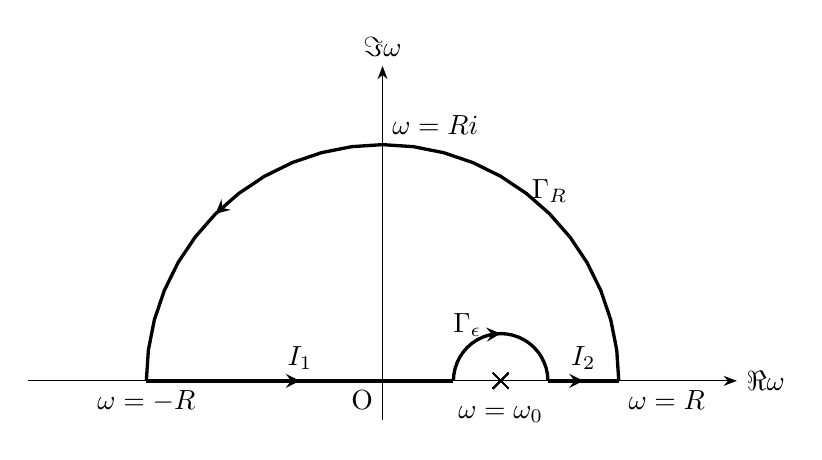
\begin{tikzpicture}[%詳細設定(気にしない)
        arrow/.style={
            postaction={
                decorate,
                decoration={
                    markings,
                    mark=at position #1 with {\arrow{stealth}}
                  }
              }
          },label2/.style 2 args={
            pos/.style={
                postaction={
                    decorate,
                    decoration={
                        markings,
                        mark=at position ##1 with \node #2;
                      }
                  }
              }
          },label/.style={
            label2={1}{#1}
          },pos/.default=.5
        ,arrow/.default=.5
      ]

      % 複素数平面の描画
      \draw[-{Stealth}] (-4.5,0) -- (4.5,0) node[right]{$\Re \omega$};
      \draw[-{Stealth}] (0,-0.5) -- (0,4) node[above]{$\Im \omega$};
      % 原点の描画
      \draw (0,0) node[below left]{O};

      % 座標の定義
      \coordinate (min_Rw) at (-3, 0);
      \coordinate (left_cutoff) at (0.9, 0);
      \coordinate (right_cutoff) at (2.1, 0);
      \coordinate (max_Rw) at (3, 0);
      \coordinate (top) at (0, 3);
      \coordinate (singular) at (1.5, 0);
      % 座標の描画
      \draw (min_Rw) node[below] {$\omega=-R$};
      \draw (max_Rw) node[below right] {$\omega=R$};
      \draw (top) node[above right] {$\omega=Ri$};
      \draw (singular) node[below=0.2cm] {$\omega=\omega_0$};

      % 特異点
      \draw[
        only marks,
        mark=x,
        mark size=4pt
      ] plot (singular);

      % 直線経路
      \draw[
        very thick,
        arrow
      ] (min_Rw) -- (left_cutoff) node[midway,above] {$I_1$};
      \draw[
        very thick,
        arrow=.5
      ]  (right_cutoff) -- (max_Rw) node[midway,above] {$I_2$};

      % 円弧経路
      \draw[
        very thick,
        domain=0:180,
        variable=\t,
        label={[above]{$\Gamma_R$}},
        pos={.25},
        arrow=.75
      ] plot ({3*cos(\t)},{3*sin(\t)});%pos,arrowの両方ともに省略していない
      \draw[
        very thick,
        domain=180:0,
        variable=\t,
        label={[above]{$\Gamma_\epsilon$}},
        pos={.25},
        arrow=.5
      ]  plot ({1.5+0.6*cos(\t)},{0.6*sin(\t)});%両方ともに省略していない

    \end{tikzpicture}
    \caption{遅延グリーン関数の積分経路}\label{fig:retarded_green_function}
  \end{center}
\end{figure}
% textlint-enable


\newpage
\bibliography{reference}

\end{document}